\documentclass{ctexart}
\usepackage{ctex}
\usepackage{graphicx}
\usepackage{amsmath}
\usepackage{amsfonts}
\usepackage{listings}

\graphicspath{{figures/}}

\title{深度学习}
\author{Mr Wu}
\date{\today}

\begin{document}
	\maketitle
	\section{卷积神经网络}
	\subsection{为什么用CNN处理图像?}
	属性一、有些模式比整个图片小很多,一个神经元不需要看到整个图像就可以识别这些模式。因此连接到一个小区域就足够了,也对应着更少的参数。
	
	属性二、有些模式出现在图片中不同的区域,可以使用相同的参数来处理它们。
	
	属性三、子抽样不会改变目标。
	\subsection{Convolution}
	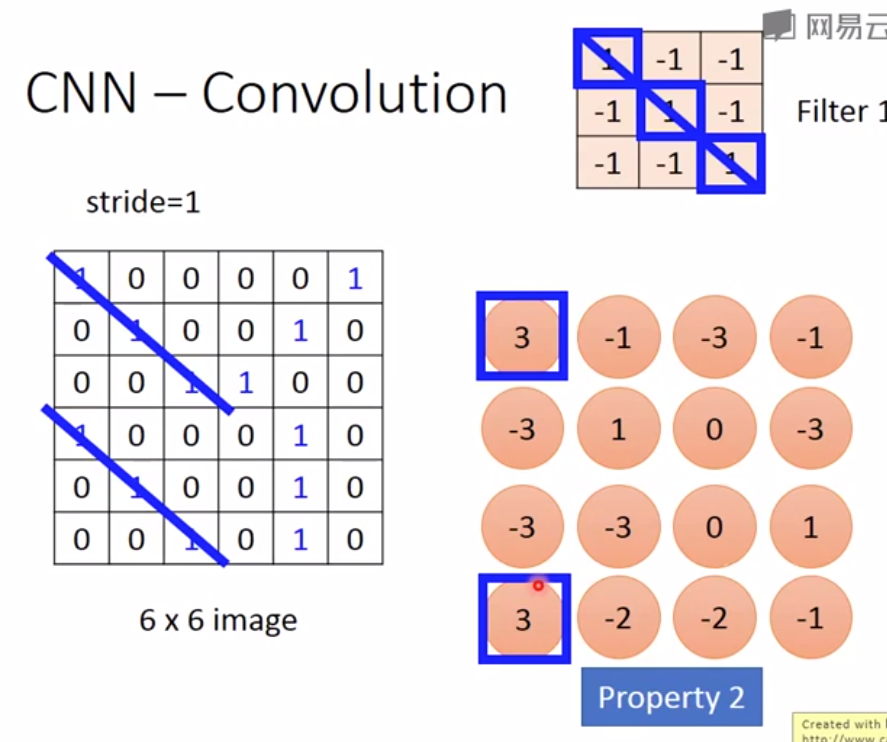
\includegraphics[scale=0.5]{1}
	
	如上图,原始图片为$ 6 \times 6 $,filter为$ 3 \times 3 $。用一个filter首先对应原始图片中左上角的$ 3 \times 3 $的区域,然后做卷积,即对应元素相乘,最终得到一个结果3.这个数字越大,就表明原始图片中的这一小块区域越贴合从左上到右下的这条斜线的特征。这就对应着上面说的属性一:一个神经元只需要看到图像的一部分就可以识别某些模式。
	
	然后向右移动这个filter,继续上面的操作。再往下移动,直到遍历了原始图片的所有区域为止。最终我们得到一个$ 4 \times 4 $的矩阵。注意左下角也有一个3,和左上角一样。这就对应了上面的属性二:有些模式出现在图片中不同的区域,所以用同一个filter就可以检测到。
	\subsection{彩色图像}
	\subsection{卷积VS全连接}
	卷积只连接了部分点。比如原始图片有36个像素点,对于最后结果$ 4 \times 4 $的矩阵,左上角的3只连接了原始图片中的第1,2,3;7.8.9;13.14.15个像素点,因此使用了更少的参数。
	\subsection{Max Pooling}
	\section{RNN}
	\section{GCN}
\end{document}